\documentclass{../src/bcthesispart}
\title{Mathematical details of Dirichlet-categorical naming game}
\author{Bas Cornelissen}
\begin{document}

%——————————————————————————————————————————————————————————
\appendixtitle{Mathematical details of Dirichlet-categorical naming game}%
	{Mathematical details of Dirichlet-categorical naming game}%
	{bng-math}{% 
	%
	% Abstract
	% ————————
	This appendix develops the Dirichlet-categorical naming game in a more rigorous fashion. Please refer to chapter \ref{ch:bayesian-naming-game} for extensive motivation.
	}
%——————————————————————————————————————————————————————————

	
	
\noindent
First, recall our notational conventions.
The most precise notation would be of the form
%-
\begin{align}
	\vect \alpha_A^{(t)} 
		= \Bigl(\alpha_{A,1}^{(t)}, \dots, \alpha_{A, K}^{(t)}\Bigr) 
		\in\mathbb{R}^K,
\end{align}
%-
and indicates the agent, the time and indices. I nearly always prefer a cleaner notation and often drop agents, or even time indices, whenever they are irrelevant.
Also, vectors (boldface) get their time index in the subscript.
Further recall that $\vectsum{\vect\alpha} := \sum_k \alpha_k$ and that we write $\ind{ \text{ condition }}$ for the indicator function evaluating to 1 if the condition holds and to 0 otherwise




%——————————————————————————————————————————————————————————
\subsection{The Dirichlet and categorical distribution}

The Dirichlet distribution is a continuous multivariate probability distribution defined over the interior of the $(K-1)$-simplex which we denote as $\simplex^{K-1}= \{x \in \R^K: \sum_k \obs_k = 1 \text{ and } 0 < \obs_i < 1 \}$. 
We will only consider the $(K-1)$-simplex, so drop the superscript.
Samples of a Dirichlet can thus be interpreted as $K$-dimensional probability-vectors.
The Dirichlet is parametrised by a $K$-vector $\vect\alpha$ and its density is given by
%-
\begin{equation}
	p(\vlang \mid \vect \alpha) 
		= D(\vect\alpha)
			\prod_{k=1}^K \lang_k^{\alpha_k - 1},
	\qquad 
	D(\vect\alpha)
		= \frac{\Gamma(\vectsum{\alpha})}{\prod_{k=1}^K\Gamma(\alpha_k)}, 
\end{equation}
%-
where $D(\vect\alpha)$ is the normalising constant, computed using the gamma function $\Gamma$, a continuous extension of the factorial with $\Gamma(n+1) = n!$ for $n \in \mathbb{N}$. 
If $\vlang \sim \text{Dirichlet}(\vect\alpha)$, then it has the following properties \parencite[e.g.][]{Bishop2006}
%-
\begin{align}
	\text{E}[\lang_k] 
		&= \frac{\alpha_k}{\vectsum{\alpha}}, 
	\qquad
	\text{Var}[\lang_k] 
		=\frac{\alpha_k ( \vectsum{\alpha} - \alpha_k)}{\vectsum{\alpha}^2(\vectsum{\alpha} + 1)},
	\qquad
	\text{Mode}[\lang_k] 
		= \frac{\alpha_k - 1}{\vectsum{\alpha} - K}.
\end{align}
%-
It is often convenient to parametrise the Dirichlet differently, as $\vect \alpha := \beta \cdot \vect\mu$ with $\beta\in\mathbb{R}$ and $\vect\mu\in\simplex$.
Here $\beta$ is the concentration parameter, a kind of inverse variance, and $\vect\mu$ determines the location of the distribution. 
This translates into
%-
\begin{equation}
	\text{E}[\lang_k] = \mu_k,\qquad
	\text{Var}[\lang_k] = \frac{\mu_k(1-\mu_k)}{\beta+1}
\end{equation}
%-
from which we see that the mean is determined by $\vect\mu$ and that larger $\beta$ lead to smaller variance.
We will use both parametrisations interchangeably.




The categorical distribution is a discrete probability distribution over $K$ outcomes, described by a probability vector $\vlang \in \simplex$.
Recall that $c_k = \sum_i \ind{\obs_i = k}$ counts the number of $k$'s in $\vobs$.
The joint distribution of $b$ i.i.d.\ categorical variables $\vobs= (\obs_1, \dots, \obs_b)$ is then given by
%-
\begin{equation}
	\label{eq:app-bng:joint-iid-categoricals}
	%-----
	p(\vobs \mid \vlang)
		= \prod_{i=1}^b \prod_{k=1}^K \lang_k^{\ind{\obs_i=k}} 
		= \prod_{k=1}^K \lang_k^{\sum_i \ind{\obs_k = k}} 
		= \prod_{k=1}^K \lang_k^{c_k},
\end{equation}
%-




%——————————————————————————————————————————————————————————
\paragraph{Dirichlet-categorical distribution}

To show that the Dirichlet is the \emph{conjugate prior} of the categorical distribution, consider the following model
%-
\begin{align}
	\vlang 
		&\sim \text{Dirichlet}(\vect\alpha)
	\\
	\obs_1, \dots, \obs_b 
		&\sim \text{Categorical}(\vlang).
\end{align}

In this case, conjugacy means that the posterior distribution $p(\vlang \mid \vobs, \vect\alpha)$ is of the same parametric form as the prior $p(\vlang \mid \vect\alpha)$, namely a Dirichlet.
More precisely, we have
%-
\begin{align}
	p(\vlang \mid \vobs, \vect\alpha) 
		&\propto p(\vlang\mid \vect\alpha) \cdot p(\vobs \mid \vlang) 
		\\
		&\propto 
			\prod_{k=1}^K \lang_k^{\alpha_k - 1}
			\cdot \prod_{k=1}^K \lang_k^{c_k} 
		\\
		&= \prod_{k=1}^K \lang_k^{\alpha_k + c_k - 1}. 
			%-----	
			\label{eq:app-bng:joint-density-dirichlet}
\end{align}
%-
In the last line one can recognise a Dirichlet density with parameters $\vect\alpha + \vect c$.
We conclude that the the posterior is $\text{Dirichlet}(\vect\alpha +\vect c)$-distributed, or, more explicitly,
%-
\begin{equation}
	\vlang \mid \vobs, \vect\alpha \sim \text{Dirichlet}(\alpha_1 + c_1, \dots, \alpha_K+c_K).
\end{equation}
%-
This result also illustrates the workings of the hyperparameter $\vect\alpha$.
It is as if the model pretends to have observed $\alpha_k$ more instances of category $k$ that it actually has.
For that reason, the $\alpha_k$'s are often called \emph{pseudo-counts}.




We can also derive the compound distribution $p(x \mid \vect \alpha) = \int_{\simplex} p(x \mid \vlang)\cdot p(\vlang \mid \vect\alpha) \; d\vlang$ by marginalizing out all probability vectors $\vlang$.
To do this, we have to use a trick, which exploits the fact that the Dirichlet distribution is normalized,
%-
\begin{equation}
	\int_{\simplex} 
		D(\vect\alpha) 
		\prod_{k=1}^K \lang_k^{\alpha_k - 1} 
		\; d\vlang 
	= 1.
\end{equation}
%-
Moving the normalising constant out of the integral, we see that
%-
\begin{equation}
	\int_{\simplex} 
		\prod_{k=1}^K \lang_k^{\alpha_k - 1} 
		\; d\vlang 
	= \frac{1}{D(\vect\alpha)}
\end{equation}
%-
Using that trick we can compute the marginal probability of $\vobs$ as
%-
\begin{align}
	p(\vobs \mid \vect\alpha) 
		&= \int_{\simplex} 
				\prod_{i=1}^b p(\obs_i \mid \vlang) 
				\cdot p(\vlang \mid \vect\alpha) 
				\; d\vlang
			\\
		&= \int_{\simplex} 
				\prod_{i=1}^b \lang_{\obs_i} 
				\cdot D(\vect\alpha) 
				\cdot \prod_{k=1}^K \lang_k^{\alpha_k - 1} 
				\; d\vlang 
			\\
		&= D(\vect\alpha)
			\int_{\simplex} 
				\prod_{k=1}^K \lang_k^{\alpha_k + c_k - 1} 
				\; d\vlang 
			\\
		&= \frac{D(\vect\alpha)}%
			{D(\vect \alpha + \vect c)}
			%-----
			\label{eq:app-bng:deriv-continue}
			\\
		&= \frac{\Gamma(\vectsum{\vect\alpha})}{\Gamma(\vectsum{\vect\alpha + \vect c})}
			\prod_{k=1}^K \frac{\Gamma(\alpha_k + c_k)}{\Gamma(\alpha_k)}
			%-----
			\label{eq:app-bng:dirichlet-categorical-compound}
\end{align}
%-
Note that when $b=1$, hence $\vobs = (x)$, the (almost defining) relation $\Gamma(n+1) = n \Gamma(n)$ can be exploited to further simplify the distribution. 
Concretely, note that $\Gamma(\vectsum{\vect\alpha + \vect c}) = \Gamma(\vectsum{\vect\alpha} + 1) = \vectsum{\alpha} \Gamma(\vectsum{\vect\alpha})$. 
This simplifies the first term in equation \ref{eq:app-bng:dirichlet-categorical-compound}, so we can simplify the marginal probability to
%-
\begin{align}
	p(x \mid \vect\alpha)
		&= \frac{1}{\vectsum{\vect\alpha}}
			\cdot \frac{\Gamma(\alpha_x + 1)}{\Gamma(\alpha_x)}
			\cdot \prod_{k\neq x} \frac{\Gamma(\alpha_k)}{\Gamma(\alpha_k)}
		\\
		&= \frac{1}{\vectsum{\vect\alpha}}
			\cdot \frac{\alpha_x \Gamma(\alpha_x)}{\Gamma(\alpha_x)}
		= \frac{\alpha_x}{\vectsum{\vect\alpha}}.
\end{align}
%-
This also gives the posterior predictive distribution $p(y \mid \vobs, \vect\alpha)$, since that is just $p(y \mid \vect\alpha')$ for the updated parameters $\vect\alpha' := \vect\alpha + \vect c$:
%-
\begin{align}
	p(y \mid \vobs, \vect\alpha) 
	= \frac{\alpha_y + c_y}{\vectsum{\vect\alpha + \vect c}}
	%-----
	\label{eq:app-bng:predictive}
\end{align}
%-
This is a remarkably simple result, indeed: the probability of observing $y$ is proportional to the number of times it has been observed already, including the pseudo-observations.




%——————————————————————————————————————————————————————————
%——————————————————————————————————————————————————————————
\subsection{Exponentiated distributions}
%——————————————————————————————————————————————————————————
%——————————————————————————————————————————————————————————



Different strategies can be used for selecting languages or words in the Bayesian Naming Game.
This is done by exponentiating the distributions $p\bigl(\vlang \mid \vect\alpha\bigr)$ and $p\bigl(\vobs \mid \vlang\bigr)$ by two parameters, $\eta$ and $\zeta$ respectively.
The resulting distributions again take simple form:
%-
\begin{align}
	p(\vlang \mid \vect\alpha)^\eta
		&\propto \Bigl(\prod_{k=1}^K \lang_k^{\alpha_k - 1}\Bigr)^\eta
		= \prod_{k=1}^K \lang_k^{[\eta(\alpha_k - 1) + 1] - 1}
		\\
		&\propto \text{Dirichlet}(\vlang \mid \eta(\vect\alpha-\vect1)+\vect1).
\end{align}
%-
The case of the categorical is obvious,
%-
\begin{align}
	p\bigr(x \mid \vlang\bigl)^\zeta 
		= \frac{\lang_x^\zeta}{\vectsum{\vlang^\zeta}}.
\end{align}
%-
So we conclude that
%-
\begin{align}
	\label{eq:app-bng:exponentiated-dirichlet}
	%-----
	p_\LA\bigl(\vlang \mid \vect\alpha\bigr)
		&= \text{Dirichlet}\bigl(\vlang \mid \eta(\vect\alpha -\vect1)+\vect1\bigr)
	\\
	p_\PA\bigl(x \mid \vlang \bigr)
		&= \text{Categorical}\bigl(x \mid \vect\theta^\zeta /\vectsum{\vect\theta^\zeta}\bigr)
\end{align}
%-




%——————————————————————————————————————————————————————————
\paragraph{The difficult case $\zeta=\infty$}

Whenever $\zeta\neq1$, Bayesian agents are facing a different inference problem and should infer the posterior distribution $p(\vlang\mid\vobs, \vect\alpha)\propto p(\vobs \mid \vlang)^\zeta \cdot p(\vlang \mid\vect\alpha)$.
However, this is no longer a Dirichlet distribution. To see this, we compute the joint
\begin{align}
	p\bigl(\vlang, \vobs \mid \vect\alpha \bigr)
		&= p\bigl(\vlang \mid \vect\alpha \bigr)
			\cdot \prod_{i=1}^b p\bigr(\obs_i \mid \vlang \bigl)^\zeta
		\\
		&= D(\vect\alpha)
			\cdot \prod_k \lang_k^{\alpha_k - 1} 
			\cdot \frac{1}{\vectsum{\vlang^\zeta}}
			\cdot \prod_k\lang_k^{\zeta \cdot c_k}
		\\
		&= \frac{1}{\vectsum{\vlang^\zeta}}
			\cdot D(\vect\alpha)
			\cdot \prod_k \lang_k^{\alpha_k + \zeta c_k - 1}
\end{align}
Although this is reminiscent of the Dirichlet density, it is not proportional to it, since the first term depends on $\vlang$.
Consequently, deriving a closed-form expression of the posterior seems hard, as it involves solving the integral
\begin{equation}
	\int_\simplex 
		\frac{1}{\vectsum{\vlang^\zeta}} 
		\prod_k \lang_k^{\alpha_k + \zeta c_k -1} 
		\; d\vlang.
\end{equation}
The reciprocal of the sum hindered any progress on this point and all suggestions would be more than welcome.\footnote{%
	%>>>
		I also posted the problem at \href{math.stackexchange.com/q/2360468}{math.stackexchange.com/q/2360468}.
	%<<<
	}




This might be an interesting problem in its own, partly because we \emph{can} relatively easily identify the extreme cases.
When $\zeta=1$ we trivially get the normal posterior, but when $\zeta=\infty$ we can also get an idea of the posterior.  
After observing $x$, the language $\vlang$ used to generate it can only be one where $x$ gets maximum probability.
In other words, $\vlang$ must have been in $\simplex_x := \{\vlang \in \simplex: \lang_x \ge \lang_k \text{ for all $k$} \}$. 
Consequently,
%-
\begin{align}
	p(\vlang \mid x, \vect\alpha) 
		&= p(\vlang \mid \vlang \in \simplex_x, \vect\alpha)
		\\
		&= \frac{\ind{\vlang \in \simplex_x} \cdot \text{Dirichlet}(\vlang \mid \vect\alpha)}%
			{\int_{\simplex_x} 
				\text{Dirichlet}(\vlang \mid \vect\alpha) 
				\; d\vlang}
\end{align}
%-
That is, the posterior is proportional to the prior, restricted to the section $\simplex_x$ of the simplex where the largest component is $x$.
I have not tried integrating the Dirichlet over $\simplex_x$ yet, other than the symmetric case, i.e. $\alpha = \nicefrac{\beta}{K} \cdot \mathbb{1}$, when the integral is simply $\nicefrac{1}{K}$.
In any case, one immediately sees that this cannot be a Dirichlet distribution: the posterior is discontinuous at the boundary of $\simplex_x$, or at least at the part of it that lies inside $\simplex$.




%- - - - - - -
\begin{SCfigure}
	\includegraphics[trim=0.94cm 0 0 \figtopmargin]{{FIG02-posterior-zeta-infty}}
	\caption{The posterior distribution $p(\vlang \mid x)$ for various $x$ if $\zeta=\infty$, that is, if agents always pick the most likely word.
		The posterior restricts the prior to the area of the simplex where $\argmax_k \lang_k = x$.
		\figdetails{\figid{FIG02}}
		\label{fig:app-bng:posterior-zeta-infty}}
\end{SCfigure}
%- - - - - - -



All this is illustrated in figure \ref{fig:app-bng:posterior-zeta-infty}.
It should be clear from that figure that agents who update their beliefs like this very quickly run into serious problems.
After observing $x=0$ all mass is restricted to $\simplex_0$ and if the agent next observes $x=1$, it has the problem that $p(1 \mid \vect\alpha) = \int_{\simplex_0} p(\vlang, 1) \; d\vlang = 0$.
This is one of the reasons for assuming that agents use exaggerated distributions only during production, and do \emph{not} account for them during posterior inference.





%——————————————————————————————————————————————————————————
%——————————————————————————————————————————————————————————
\subsection{Measuring the distance between languages}
%——————————————————————————————————————————————————————————
%——————————————————————————————————————————————————————————




Most measures introduced to analyse the Dirichlet-categorical naming game, measure distances between languages.
As a distance measure for distributions, the Jensen-Shannon divergence (\textsc{jsd}) can be used.
The \textsc{jsd} is a symmetric version of the more common Kullback-Leibler divergence and measures the similarity between probability distributions.
Figure \ref{fig:app-bng:jsd} illustrates the \textsc{jsd} of different discrete distributions to the uniform distribution.
Formally, if $\vect\pi_1, \dots, \vect\pi_N$ are probability distributions, their divergence is
%-
\begin{equation}
	\textsc{jsd}(\vect\pi_1, \dots, \vect\pi_N)	
		:= H\Bigl( \frac{1}{N} \sum_{i=1}^N \vect\pi_i \Bigr)	 
			- \frac{1}{N} \sum_{i=1}^N H(\vect\pi_i),
\end{equation}
%-
where $H$ is the Shannon-entropy, a measure for the uncertainty in a distribution.
As one can see, the \textsc{jsd} measures the difference between the entropy of the average distribution and the average entropy.
If the divergence is zero, the distributions are identical since the \textsc{jsd} is the square of a metric \parencite{Endres2003,Briet2009}.
The divergence is moreover bounded,
%- 
\begin{equation}
	0 	\le \textsc{jsd}(\vect\pi_1, \dots, \vect\pi_N) 
		\le \log_2(N)	
\end{equation}
%-
so the normalised divergence, between 0 and 1, is obtained by dividing by $\log_2(N)$.




%- - - - - - -
\begin{SCfigure}
	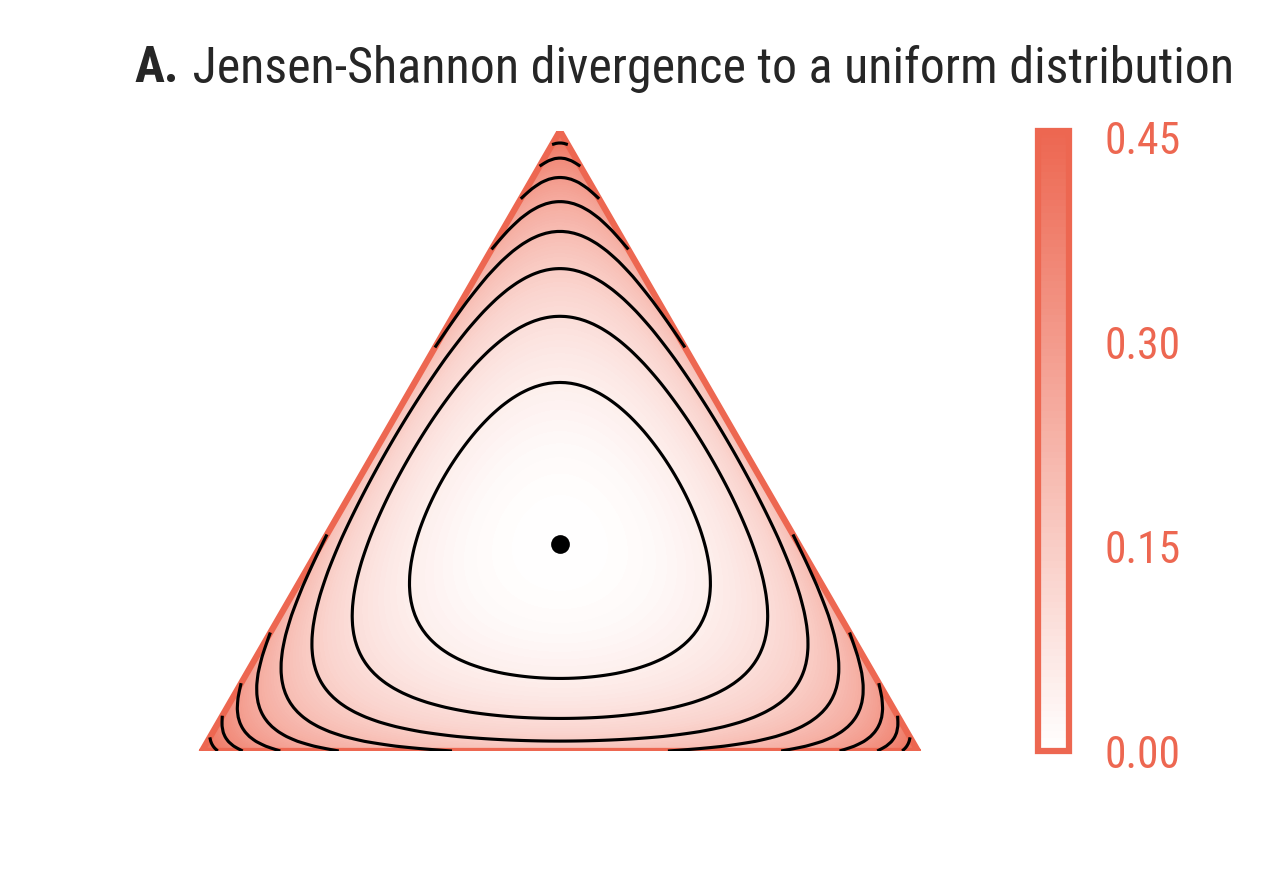
\includegraphics[trim=0.94cm 0 0 \figtopmargin]{FIG02-JSD}
	\caption{The divergence between distributions in the 2-simplex and the uniform distribution $(\nicefrac{1}{3},\nicefrac{1}{3}, \nicefrac{1}{3})$ (indicated by a dot) under the Jensen-Shannon divergence. Points on the solid lines have the same distance to the uniform \figdetails{\figid{fig02}
			Figure inspired by a blogpost of Lior Pachter \href{http://liorpachter.wordpress.com/tag/jensen-shannon-metric}{liorpachter.wordpress.com/tag/jensen-shannon-metric/}}
		\label{fig:app-bng:jsd}}
\end{SCfigure}
%- - - - - - -




%——————————————————————————————————————————————————————————
%——————————————————————————————————————————————————————————
\subsection{Bayesian updating and lateral inhibition}
%——————————————————————————————————————————————————————————
%——————————————————————————————————————————————————————————


Intuitively, Bayesian updating implements a kind of lateral inhibition — but how exactly?
We derive the ‘update’ rules in the Dirichlet-categorical naming game.
Recall that every word is assigned a score $s(x) = p(x \mid \vect \alpha)$.
The question is how score of word $y$ changes after observing $x$.
That is, what is $s_{t+1}(x)$ in terms of $s_t(x)$?
For a sampler, this follows directly from \eqref{eq:app-bng:predictive}:
%-
\begin{align}
	\label{eq:app-bng:update-sampler}
	%-----
	s_{t+1}(y) 
		= p(y \mid x, \vect\alpha)
		&= \frac{\alpha_y + \ind{y = x}}%
			{\vectsum{\vect\alpha} + 1}
		\\
		&= \frac{\alpha_y}{\vectsum{\vect\alpha}} 
			\cdot \frac{\vectsum{\vect\alpha}}%
				{\vectsum{\vect\alpha} + 1} 
			+ \frac{\ind{y = x}}%
				{\vectsum{\vect\alpha} + 1}
		\\
		&= s_t(y)
			\cdot \frac{\vectsum{\vect\alpha}}%
				{\vectsum{\vect\alpha} + 1} 
			+ \frac{\ind{y = x}}%
				{\vectsum{\vect\alpha} + 1}
\end{align}
%-




For the \textsc{map} language strategy ($\eta=\infty$), the agent always chooses the mode $\vect\nu$ of the distribution $\text{Dirichlet}(\vect\alpha)$, i.e.,
%-
\begin{equation}
	\vect\nu 
		= \frac{\vect\alpha - 1}%
			{\vectsum{\vect\alpha} - K}
\end{equation}
%-
The score $s(y) = p(y \mid x, \vect\alpha)$ is therefore the $y$’th component of the mode. 
A similar argument as above shows that
%-
\begin{align}
	\label{eq:app-bng:update-MAP}
	%-----
	s_{t+1}(y) 
		= s_t(y)
	 		\cdot \frac{\vectsum{\vect\alpha} - K}%
	 			{\vectsum{\vect\alpha} - K + 1}
			+ \frac{\ind{y=x}}%
				{\vectsum{\vect\alpha} - K + 1}.
\end{align}
%-
This is a similar lateral inhibition mechanism as the one used by samplers.



\showbibliography


\end{document}
